\PassOptionsToPackage{unicode}{hyperref}
\PassOptionsToPackage{naturalnames}{hyperref}

\documentclass[xcolor=dvipsnames, aspectratio=149, 12pt]{beamer}


\usepackage{etex}
%\usetheme{Darmstadt}
\usetheme{Madrid}
%\usecolortheme[named=NavyBlue]{structure}
\usecolortheme{whale}

%\usetheme{Frankfurt}  %\usecolortheme{default}

%\useoutertheme{infolines}

\mode<presentation>

\setbeamersize{text margin left=5mm}
\setbeamersize{text margin right=5mm}
\setbeamertemplate{footline}[page number]{}
\setbeamertemplate{blocks}[rounded][shadow=false]
\setbeamertemplate{title page}[default][colsep=-4bp,rounded=true]
\beamertemplatenavigationsymbolsempty
    %\setbeamertemplate{footline}{%
     % \raisebox{5pt}{\makebox[\paperwidth]{\hfill\makebox[10pt]{\scriptsize\insertframenumber}}}}
      
\addtobeamertemplate{block begin}{\setlength{\textwidth}{0.99\textwidth}}{}
\addtobeamertemplate{block begin}{\setlength\abovedisplayskip{0pt}}
%\addtobeamertemplate{block begin}{\vspace{-25pt}}{}


\usepackage{ucs}
\usepackage[utf8x]{inputenc}
\usepackage[greek,english]{babel}
\newcommand{\en}{\selectlanguage{english}}
\newcommand{\el}{\selectlanguage{greek}}
\usepackage[T1]{fontenc}
\usepackage{lmodern}

\usepackage[absolute,overlay]{textpos}

\newcommand{\sq}{\selectlanguage{english}\color{red!70!blue}\bf}
\newcommand{\bb}{\selectlanguage{greek}\color{blue!50!black}\bf}
\newcommand{\ra}{\selectlanguage{english}\color{blue!90!red}\em\large}
\newcommand{\enb}{\selectlanguage{english}\color{blue}}
\newcommand{\ex}[1]{\begin{math}\partial{#1}\end{math}}

\newcommand{\cgg}{\selectlanguage{english}\color{green!60!black}\bf}
\newcommand{\cmm}{\selectlanguage{english}\color{red!50!blue}\bf}

\newcommand{\cee}{\selectlanguage{greek}\color{red!90!blue}\bf\large}
\newcommand{\bbl}{\color{blue!90!black}\bf}
\newcommand{\crr}{\color{red!90!blue}\bf}
\newcommand{\cbb}{\color{blue!90!black}\bf}

\colorlet{colBC}{Apricot!50}

%\usepackage{enumitem}
\usepackage{booktabs}
\usepackage{hyperref}
\usepackage{listings}
\usepackage{fancyvrb}
\usepackage{listings}
\usepackage{amsmath}
\usepackage{amssymb}
\usepackage{mathtools}
\usepackage{mathrsfs}
\usepackage{colortbl}
\usepackage{graphicx}
\usepackage{chngcntr}
%\usepackage{subfig}
%\usepackage{subcaption}}
\usepackage{pgf, tikz}
\usepackage{pgfplots} %\pgfplotsset{compat=newest}
\usepackage{pgfplotstable}
\usepackage{comment}
\usepackage[normalem]{ulem}

\usepackage[tikz]{bclogo}
\usetikzlibrary{matrix}
\usetikzlibrary{arrows,automata,shapes,calc,positioning,fit}
\usetikzlibrary{backgrounds,shadows,trees}


\usetikzlibrary{calc}
%\usepackage{booktabs}
\usepackage{attachfile}

\definecolor{blue10}{RGB}{135, 204, 255}
\definecolor{blue90}{RGB}{0, 0, 204}


\DefineVerbatimEnvironment{codeE}{Verbatim}
{
  frame            = leftline,
  samepage         = true,
  commandchars     = &\{\}, 
  rulecolor=\color{black!50!white}, framerule=3px,
  baselinestretch  = 1,
  fontsize         = \small
}

\DefineVerbatimEnvironment{codeR}{Verbatim}
{
  frame            = leftline,
  samepage         = true,
  numbers          = left,
  numbersep        = 6pt,
  commandchars     = &\{\}, 
  rulecolor=\color{red!90!black}, framerule=3px,
  baselinestretch  = 1,
  fontsize         = \small
}

\DefineVerbatimEnvironment{codeM}{Verbatim}
{
  frame=leftline,  framerule=2px,  rulecolor=\color{blue},
  samepage=true, numbers=left,   numbersep=6pt,
  commandchars=&\{\}, baselinestretch=1, fontsize=\small
}

\DefineVerbatimEnvironment{codeO}{Verbatim}
{
  frame=leftline,  framerule=2px,  rulecolor=\color{blue},
  samepage=true, numbers=left,   numbersep=6pt,
  commandchars=&\{\}, baselinestretch=1, fontsize=\small
}

\DefineVerbatimEnvironment{SQL}{Verbatim}
{
  frame=leftline,  framerule=2px,  rulecolor=\color{blue},
  samepage=true, numbers=left,   numbersep=6pt,
  commandchars=&\{\}, baselinestretch=1, fontsize=\small
}

\DefineVerbatimEnvironment{codeC}{Verbatim}
{
  frame=leftline,  framerule=2px,  rulecolor=\color{blue},
  samepage=true, numbers=left,   numbersep=6pt,
  commandchars=&\{\}, baselinestretch=1, fontsize=\small
}


\newcommand{\code}[1]{\en \textsl{#1}}{\el}
\newcommand{\ojoinaux}{\setbox0=\hbox{$\bowtie$}%
  \rule[-.02ex]{.25em}{.4pt}\llap{\rule[\ht0]{.25em}{.4pt}}}
\newcommand{\ojoin}{\mathbin{\ojoinaux\mkern-5.6mu\bowtie\mkern-5.7mu\ojoinaux}}
\newcommand{\lojoin}{\mathbin{\ojoinaux\mkern-5.6mu\bowtie}}
\newcommand{\rojoin}{\mathbin{\bowtie\mkern-5.7mu\ojoinaux}}

\newcommand{\stirlingtwo}[2]{\genfrac{\lbrace}{\rbrace}{0pt}{}{#1}{#2}}

\logo{\includegraphics[width=2.5cm,height=2.5cm,keepaspectratio]{../common/SQL2.jpg}}

\AtBeginSection[]
{ \el
  \begin{frame}<beamer>
    \frametitle{Περιεχόμενα}
    \begin{minipage}{\wE}
      \tableofcontents[currentsection]
    \end{minipage} 
  \end{frame}
}

\AtBeginSubsection[]
{
  \begin{frame}<beamer>
    \frametitle{Περιεχόμενα}
    \begin{minipage}{\wE}
      \tableofcontents[currentsubsection]
    \end{minipage}   
  \end{frame}
}


\newcommand{\wE}{0.88\textwidth}
\newcommand{\wN}{0.92\textwidth}



\newcommand{\men}[1] {\selectlanguage{english}#1\selectlanguage{greek}}
\newcommand{\mene}[1] {\selectlanguage{english}\emph{#1}\selectlanguage{greek}}
\newcommand{\mgr}[1] {\selectlanguage{greek}#1\selectlanguage{english}}
\newcommand{\mgre}[1] {\selectlanguage{greek}\emph{#1}\selectlanguage{english}}


% η \tsql τυπώνει SQL
\newcommand{\tsql}{\selectlanguage{english}SQL\selectlanguage{greek}}
\newcommand{\tasql}{\selectlanguage{english}ANSI-SQL\selectlanguage{greek}}
\newcommand{\tddl}{\selectlanguage{english}DDL\selectlanguage{greek}}
\newcommand{\tdml}{\selectlanguage{english}DML\selectlanguage{greek}}

\newcommand{\tselect}{\selectlanguage{english}SELECT\selectlanguage{greek}}
\newcommand{\tselectd}{\selectlanguage{english} SELECT$\ldots$ \selectlanguage{greek}}
\newcommand{\tfrom}{\selectlanguage{english}FROM\selectlanguage{greek}}
\newcommand{\tfromd}{\selectlanguage{english} FROM$\ldots$ \selectlanguage{greek}}
\newcommand{\twhere}{\selectlanguage{english}WHERE\selectlanguage{greek}}
\newcommand{\twhered}{\selectlanguage{english} WHERE $\ldots$\selectlanguage{greek}}
\newcommand{\torderby}{\selectlanguage{english}ORDER BY\selectlanguage{greek}}
\newcommand{\tgroupby}{\selectlanguage{english}GROUP BY\selectlanguage{greek}}
\newcommand{\thaving}{\selectlanguage{english}HAVING\selectlanguage{greek}}
\newcommand{\trollup}{\selectlanguage{english}ROLLUP\selectlanguage{greek}}
\newcommand{\tnull}{\selectlanguage{english}NULL\selectlanguage{greek}}
\newcommand{\tunk}{\selectlanguage{english}UNK\selectlanguage{greek}}
\newcommand{\tnotnull}{\selectlanguage{english}NOT NULL\selectlanguage{greek}}
\newcommand{\ttrue}{\selectlanguage{english}TRUE\selectlanguage{greek}}
\newcommand{\tfalse}{\selectlanguage{english}FALSE\selectlanguage{greek}}
\newcommand{\tlike}{\selectlanguage{english}LIKE\selectlanguage{greek}}
\newcommand{\tand}{\selectlanguage{english}AND\selectlanguage{greek}}
\newcommand{\tor}{\selectlanguage{english}OR\selectlanguage{greek}}
\newcommand{\tnot}{\selectlanguage{english}NOT\selectlanguage{greek}}
\newcommand{\tdistinct}{\selectlanguage{english}DISTINCT\selectlanguage{greek}}
\newcommand{\tavg}{\selectlanguage{english}AVG()\selectlanguage{greek}}
\newcommand{\tsum}{\selectlanguage{english}SUM()\selectlanguage{greek}}
\newcommand{\tmin}{\selectlanguage{english}MIN()\selectlanguage{greek}}
\newcommand{\tmax}{\selectlanguage{english}MAX()\selectlanguage{greek}}
\newcommand{\tcount}{\selectlanguage{english}COUNT()\selectlanguage{greek}}
\newcommand{\tcounta}{\selectlanguage{english}COUNT(*)\selectlanguage{greek}}
\newcommand{\tall}{\selectlanguage{english}ALL\selectlanguage{greek}}
\newcommand{\tany}{\selectlanguage{english}ANY\selectlanguage{greek}}
\newcommand{\texists}{\selectlanguage{english}EXISTS\selectlanguage{greek}}
\newcommand{\tdefault}{\selectlanguage{english}DEFAULT\selectlanguage{greek}}
\newcommand{\tconstraint}{\selectlanguage{english}CONSTRAINT\selectlanguage{greek}}
\newcommand{\tondelcas}{\selectlanguage{english}ON DELETE CASCADE\selectlanguage{greek}}
\newcommand{\tonupcas}{\selectlanguage{english}ON UPDATE CASCADE\selectlanguage{greek}}

\newcommand{\tjoin}{\selectlanguage{english}JOIN\selectlanguage{greek}}

\newcommand{\tinsert}{\selectlanguage{english}INSERT\selectlanguage{greek}}
\newcommand{\tdelete}{\selectlanguage{english}DELETE\selectlanguage{greek}}
\newcommand{\tupdate}{\selectlanguage{english}UPDATE\selectlanguage{greek}}

\newcommand{\tcreatedb}{\selectlanguage{english}CREATE DATABASE\selectlanguage{greek}}
\newcommand{\tcreatetab}{\selectlanguage{english}CREATE TABLE\selectlanguage{greek}}
\newcommand{\taltertab}{\selectlanguage{english}ALTER TABLE\selectlanguage{greek}}
\newcommand{\tprikey}{\selectlanguage{english}PRIMARY KEY\selectlanguage{greek}}
\newcommand{\tforkey}{\selectlanguage{english}FOREIGN KEY\selectlanguage{greek}}
\newcommand{\tdropt}{\selectlanguage{english}DROP TABLE\selectlanguage{greek}}
\newcommand{\tdropv}{\selectlanguage{english}DROP VIEW\selectlanguage{greek}}

\newcommand{\tgrant}{\selectlanguage{english}GRANT\selectlanguage{greek}}
\newcommand{\trevoke}{\selectlanguage{english}REVOKE\selectlanguage{greek}}

\newcommand{\tmysql}{\selectlanguage{english}MySQL\selectlanguage{greek}}
\newcommand{\taccess}{\selectlanguage{english}MS ACCESS\selectlanguage{greek}}
\newcommand{\toracle}{\selectlanguage{english}ORACLE\selectlanguage{greek}}
\newcommand{\tsybase}{\selectlanguage{english}Sybase\selectlanguage{greek}}
\newcommand{\tapache}{\selectlanguage{english}Apache\selectlanguage{greek}}
\newcommand{\tphp}{\selectlanguage{english}PHP\selectlanguage{greek}}


\newcommand{\tunion}{\selectlanguage{english}UNION\selectlanguage{greek}}
\newcommand{\tuniona}{\selectlanguage{english}UNION ALL\selectlanguage{greek}}
\newcommand{\tuniond}{\selectlanguage{english}UNION DISTINCT\selectlanguage{greek}}
\newcommand{\tintersect}{\selectlanguage{english}INTERSECT\selectlanguage{greek}}

\newcommand{\tcom}{$=,<>,<,<=,>,>=$}

\newcommand{\kb}{\selectlanguage{english}KBytes\selectlanguage{greek}}
\newcommand{\mb}{\selectlanguage{english}MBytes\selectlanguage{greek}}
\newcommand{\gb}{\selectlanguage{english}GBytes\selectlanguage{greek}}

\newcommand{\tdbms}{Σύστημα Διαχείρισης Βάσεων Δεδομένων}
\newcommand{\trdbms}{Σχεσιακό Σύστημα Διαχείρισης Βάσεων Δεδομένων}
\newcommand{\tdbmsg}{Συστήματος Διαχείρισης Βάσεων Δεδομένων}
\newcommand{\tdbmss}{Συστήματα Διαχείρισης Βάσεων Δεδομένων}
\newcommand{\trdbmss}{Σχεσιακά Συστήματα Διαχείρισης Βάσεων Δεδομένων}
\newcommand{\terd}{Διάγραμμα Οντοτήτων/Συσχετίσεων}
\newcommand{\terdb}{Διαγράμματος Οντοτήτων/Συσχετίσεων}
\newcommand{\ter}{Οντοτήτων/Συσχετίσεων}

\newcommand{\tcompany}{\selectlanguage{english}{\bf COMPANY}\selectlanguage{greek}}
\newcommand{\temployees}{\selectlanguage{english}\emph{employees}\selectlanguage{greek}}
\newcommand{\tdepartments}{\selectlanguage{english}\emph{departments}\selectlanguage{greek}}
\newcommand{\tprojects}{\selectlanguage{english}\emph{projects}\selectlanguage{greek}}
\newcommand{\tworkson}{\selectlanguage{english}\emph{workson}\selectlanguage{greek}}

\newcommand{\tdepid}{\selectlanguage{english}\emph{depid}\selectlanguage{greek}}
\newcommand{\tdepname}{\selectlanguage{english}\emph{depname}\selectlanguage{greek}}
\newcommand{\tmanager}{\selectlanguage{english}\emph{manager}\selectlanguage{greek}}

\newcommand{\tempid}{\selectlanguage{english}\emph{empid}\selectlanguage{greek}}
\newcommand{\tfirstname}{\selectlanguage{english}\emph{firstname}\selectlanguage{greek}}
\newcommand{\tlastname}{\selectlanguage{english}\emph{lastname}\selectlanguage{greek}}
\newcommand{\tsalary}{\selectlanguage{english}\emph{salary}\selectlanguage{greek}}
%\newcommand{\thiredate}{\selectlanguage{english}\emph{hiredate}}\selectlanguage{greek}}

\newcommand{\tproid}{\selectlanguage{english}\emph{proid}\selectlanguage{greek}}
\newcommand{\ttitle}{\selectlanguage{english}\emph{title}\selectlanguage{greek}}
\newcommand{\tbudget}{\selectlanguage{english}\emph{budget}\selectlanguage{greek}}


\newcommand{\attention}{\marginpar{\hfill\fbox{\Large{!}}}}
\newcommand{\tthink}{\selectlanguage{english} \textbf{\emph{Think in SQL and have a great fun!}} \selectlanguage{greek}}


\newcommand{\logomysql}{\marginpar{\hfill{\includegraphics[scale=0.7]{mysql.jpg}}}}
\newcommand{\logoaccess}{\marginpar{\hfill{\includegraphics[scale=0.7]{access.jpg}}}}
\newcommand{\logooracle}{\marginpar{\hfill{\includegraphics[scale=0.8]{oracle.jpg}}}}

\newcommand{\igok}    {\includegraphics[scale=1.0] {pics/OK.png}}
\newcommand{\igcancel}{\includegraphics[scale=1.0] {pics/cancel.png}}
\newcommand{\igadd}   {\includegraphics[scale=1.0] {pics/add.png}}
\newcommand{\igclose} {\includegraphics[scale=1.0] {pics/close.png}}

\newcommand{\calg} {\mathscr{G}}

\newcommand{\tsummary} {\clearpage  \section{\el Περίληψη κεφαλαίου}} 
\newcommand{\tautoeval} {\clearpage  \section{\el Ερωτήσεις αυτοαξιολόγησης}} 
\newcommand{\trepeatexer} {\clearpage  \section{\el Ασκήσεις επανάληψης}} 

\newcommand{\nf} {κανονική μορφή} 
\newcommand{\anf} {1\textsuperscript{η} κανονική μορφή} 
\newcommand{\bnf} {2\textsuperscript{η} κανονική μορφή} 
\newcommand{\cnf} {3\textsuperscript{η} κανονική μορφή} 
\newcommand{\bcnf} {\men{Boyce--Codd} κανονική μορφή} 
\newcommand{\dnf} {4\textsuperscript{η} κανονική μορφή}
\newcommand{\enf} {5\textsuperscript{η} κανονική μορφή}
\newcommand{\fnf} {6\textsuperscript{η} κανονική μορφή}   


\newcommand{\maxcard}{\mathop{\mathrm{maxcard}}}
\newcommand{\mincard}{\mathop{\mathrm{mincard}}}
 


\begin{document}
\author[]{Αθανάσιος Σταυρακούδης}
\title[]{Ερωτήματα {\en SQL} με σύζευξη πινάκων}
\date[]{Άνοιξη 2016}
\institute{\en \texttt{http://stavrakoudis.econ.uoi.gr \\ astavrak@uoi.gr \\ @AStavrakoudis}}


\el
\titlepage

\section[]{\textgreek{Γενικά για τη σύζευξη πινάκων}}


\begin{frame}[t, fragile, shrink]
\frametitle{Σκοπός του μαθήματος}
\begin{minipage}{\wE}
\begin{enumerate} \itemsep 9pt % [<+->] \pause \large
  \item Εκτελείτε ερωτήματα ανάσυρσης δεδομένων από πολλούς πίνακες.
  \item Εκτελείτε ερωτήματα που αντιστοιχούν στις σχεσιακές πράξεις καρτεσιανού γινομένου
        και σύζευξης.
  \item Εφαρμόζετε κατάλληλες συνδέσεις ({\sq JOIN}) πινάκων.        
  \item Αντιληφθείτε τις διαφορές και ομοιότητες ανάμεσα στους διαφορετικούς τύπους
        συζεύξεων.
\end{enumerate}
\end{minipage}
\end{frame}


\begin{frame}[t, fragile, shrink]
\frametitle{Το σχήμα της βάσης {\en company}}
\begin{align*}
  departments & (\underline{depid}, depname, manager) \\
  employees   & (\underline{empid}, firstname, lastname, depid, salary, hiredate) \\
  projects    & (\underline{proid}, title, budget, startdate, enddate, progress) \\
  workson     & (\underline{empid}, \underline{proid})
\end{align*}
\begin{itemize}
  \item {\ra departments}, τα τμήματα της εταιρείας
  \item {\ra employees}, οι υπάλληλοι της εταιρείας
  \item {\ra projects}, τα έργα που εκτελεί η εταιρεία
  \item {\ra workson}, η απασχόληση των υπαλλήλων στα έργα
\end{itemize}
\end{frame}



\begin{frame}[t, fragile, shrink]
\frametitle{Το σχήμα της βάσης {\en company}}
\begin{minipage}{\wE}
\begin{columns}[t]
\begin{column}{0.55\linewidth}
\begin{center}
\includegraphics[scale=0.5]{../common/companyER.png}
\end{center}
\end{column}
\begin{column}{0.4\linewidth}
\begin{center}
\begin{itemize}
  \item {\ra departments}, τα τμήματα της εταιρείας
  \item {\ra employees}, οι υπάλληλοι της εταιρείας
  \item {\ra projects}, τα έργα που εκτελεί η εταιρεία
  \item {\ra workson}, η απασχόληση των υπαλλήλων στα έργα
\end{itemize}
\end{center}
\end{column}
\end{columns}
\end{minipage}
\end{frame}


\begin{frame}[t, fragile, shrink]
\frametitle{Πρωτεύοντα και ξένα κλειδιά}
\begin{minipage}{\wE}
\begin{enumerate} \itemsep 6pt % [<+->] \pause
  \item Κάθε πίνακας έχει ένα {\crr πρωτεύον κλειδί}.
  \item Το {\crr πρωτεύον κλειδί} μπορεί να είναι απλό (ένα πεδίο), ή σύνθετο
        (συνδυασμός πεδίων).
  \item Κάθε εγγραφή ενός πίνακα μπορεί να προσδιοριστεί με τη χρήση του
        πρωτεύοντος κλειδιού.
  \item Η σύνδεση δεδομένων από διαφορετικούς πίνακες {\bbl σύζευξη}
        γίνεται (συνήθως) με τη χρήση του {\crr ξένου κλειδιού},
  \item Ένας πίνακας μπορεί να έχει πολλά ξένα κλειδιά ή  να μην έχει κανένα.
\end{enumerate}
\end{minipage}
\end{frame}


\begin{frame}[t, fragile, shrink]
\frametitle{Συσχέτιση {\en departments} και {\en employees} Ν:1}
\begin{itemize} \itemsep 6pt
  \item Ο πίνακας {\ra departments} έχει {\crr πρωτεύον κλειδί} το πεδίο {\ra depid}.
  \item Ο πίνακας {\ra employees} έχει {\crr πρωτεύον κλειδί} το πεδίο {\ra empid}.
  \item Ο πίνακας {\ra employees} έχει {\crr ξένο κλειδί} το πεδίο {\ra depid},
        το οποίο παίρνει τιμές που {\bbl αναφέρονται} στις τιμές του πεδίου
        {\ra depid} του πίνακα {\ra departments}:
        \[ departments.depid = employees.depid \]
\end{itemize}
\pause
\begin{minipage}{\wE}
\begin{itemize} 
  \item Το πεδίο {\ra employees.depid}  {\crr δεν είναι πρωτεύον κλειδί}
        και δεν παίρνει μοναδικές τιμές: πολλοί υπάλληλοι εργάζονται
        στο ίδιο τμήμα.
  \item Οι πίνακες {\ra departments} και {\ra employees}  συσχετίζονται μεταξύ τους
        με συσχέτιση {\cee Πολλά προς Ένα}.
\end{itemize}
\end{minipage}
\end{frame}


\begin{frame}[t, fragile, shrink]
\frametitle{Συσχέτιση {\en departments - employees} }
\includegraphics[scale=0.65]{company1-relationship.jpg} \\
\bigskip
\begin{minipage}{\wE}

\end{minipage}
\end{frame}

\begin{frame}[t, fragile, shrink]
\frametitle{Συσχέτιση {\en departments} και {\en employees} 1:1}
\begin{itemize}
  \item Ο πίνακας {\ra departments} έχει {\cee πρωτεύον κλειδί} το πεδίο {\ra depid}.
  \item Ο πίνακας {\ra employees} έχει {\cee πρωτεύον κλειδί} το πεδίο {\ra empid}.
  \item Ο πίνακας {\ra departments} έχει {\cee ξένο κλειδί} το πεδίο {\ra manager},
        το οποίο παίρνει τιμές που {\bbl αναφέρονται} στις τιμές του πεδίου
        {\ra empid} του πίνακα {\ra employees}:
        \[ departments.manager = employees.empid \]
\end{itemize}
\pause
\begin{minipage}{\wE}
\begin{itemize} 
  \item Το πεδίο {\ra departments.manager}  {\cee δεν είναι πρωτεύον κλειδί}
        αλλά παίρνει μοναδικές τιμές ({\sq UNIQUE}).
  \item Οι πίνακες {\ra departments} και {\ra employees}  συσχετίζονται μεταξύ τους
        με συσχέτιση {\cee  Ένα προς Ένα}.
\end{itemize}
\end{minipage}
\end{frame}




\begin{frame}[t, fragile, shrink]
\frametitle{Συσχέτιση {\en employees} και {\en projects} Ν:Ν}
\begin{minipage}{\wE}
\begin{enumerate} \itemsep 6pt % [<+->] \pause 
  \item Ο πίνακας {\ra projects} έχει {\crr πρωτεύον κλειδί} το πεδίο {\ra proid}.
  \item Ο πίνακας {\ra workson} έχει {\crr πρωτεύον κλειδί} το συνδυασμό των πεδίων
        {\ra empid} και  {\ra proid} ({\crr σύνθετο κλειδί}).
  \item Το πεδίο {\ra empid} είναι {\cee ξένο κλειδί} στον πίνακα {\ra workson}
        και αναφέρεται στο πεδίο {\ra employees.empid}.
  \item Το πεδίο {\ra proid} είναι {\crr ξένο κλειδί} στον πίνακα {\ra workson}
        και αναφέρεται στο πεδίο {\ra projects.proid}.  
  \item Ένας υπάλληλος απασχολείται σε πολλά έργα, ένα έργο απασχολεί
        πολλούς υπαλλήλους,  επομένως η συσχέτιση είναι {\cee Πολλά προς Πολλά}.
  \item Η σύζευξη των πινάκων {\ra employees} και {\ra projects} \\ γίνεται
        μέσω του πίνακα {\ra workson}.
\end{enumerate}
\end{minipage}
\end{frame}



\begin{frame}[t, fragile, shrink]
\frametitle{Το σχήμα της βάσης {\en company (MySQL)}}
\begin{minipage}{\wE}
\begin{columns}
\begin{column}{0.55\linewidth}
\begin{center}
\includegraphics[scale=0.5]{../common/companyER.png}
\end{center}
\end{column}
\begin{column}{0.4\linewidth}
\begin{center}
\begin{itemize}
  \item {\ra departments}, τα τμήματα της εταιρείας
  \item {\ra employees}, οι υπάλληλοι της εταιρείας
  \item {\ra projects}, τα έργα που εκτελεί η εταιρεία
  \item {\ra workson}, η απασχόληση των υπαλλήλων στα έργα
\end{itemize}
\end{center}
\end{column}
\end{columns}
\end{minipage}
\end{frame}


\begin{frame}[t, fragile, shrink]
\frametitle{Το σχήμα της βάσης {\en company (.odp)} }
\includegraphics[scale=0.65]{../common/company1-REL-odp.png} \\
\bigskip
\begin{minipage}{0.92\textwidth}
\begin{itemize} \itemsep 9pt
  \item {\ra departments}, τα τμήματα της εταιρείας
  \item {\ra employees}, οι υπάλληλοι της εταιρείας
  \item {\ra projects}, τα έργα που εκτελεί η εταιρεία
  \item {\ra workson}, η απασχόληση των υπαλλήλων στα έργα
\end{itemize}
\end{minipage}
\end{frame}

\section[]{\textgreek{Καρτεσιανό γινόμενο και θ σύζευξη}}



\begin{frame}[t, fragile, shrink]
\frametitle{Καρτεσιανό γινόμενο}
\begin{minipage}{\wE}
\begin{block}{Καρτεσιανό γινόμενο:}
Ο συνδυασμός των πινάκων {\ra departments} και {\ra employees}
\[
departments \times employees
\]
λέγεται καρτεσιανό γινόμενο, και περιλαμβάνει όλους τους συνδυασμούς των
εγγραφών των πινάκων {\ra departments} και {\ra employees}.
\pause
\begin{itemize}
  \item Στο αποτέλεσμα περιλαμβάνονται όλα τα πεδία των πινάκων
        {\ra departments} και {\ra employees}.
  \item Οι εγγραφές του αποτελέσματος περιλαμβάνει όλους τους συνδυασμούς των εγγραφών
        των πινάκων {\ra departments} και {\ra employees}.
\end{itemize}  
\end{block}
\end{minipage}
\end{frame}


\begin{frame}[t, fragile, shrink]
\frametitle{Καρτεσιανό γινόμενο $departments \times employees$}
%\begin{minipage}{\wE}
\begin{itemize}
  \item Όλες οι δυνατές συνδέσεις ανάμεσα στα τμήματα και σε δείγμα 3 υπαλλήλων.
  \item Μόνο οι {\crr κόκκινες γραμμές} αντιστοιχούν στην πραγματικότητα: \\ (1, 109), (6, 102), (2,153).
  \item Τα καρτεσιανό γινόμενο απεικονίζει όλα τα {\bbl πιθανά ενδεχόμενα},
        όχι απαραίτητα τα {\bbl πραγματικά γεγονότα}.
\end{itemize}
%\end{minipage}
\en
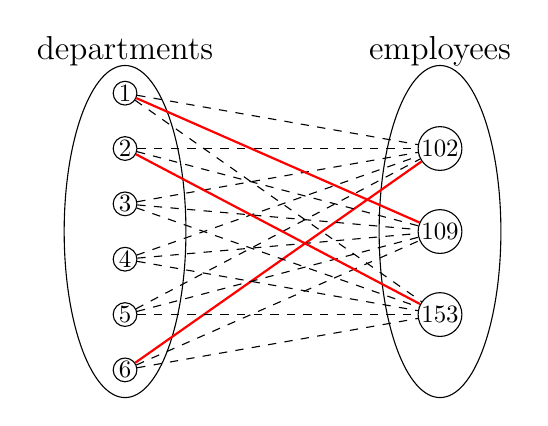
\begin{tikzpicture}
  \tikzstyle{every state} = [fill, draw=black, blue!50, text=black]
  \tikzstyle{every state} = [inner sep=0.5pt, minimum size=0pt, scale=0.9]
   
  \def\A{0.0};
  \def\B{4.0};

  \draw (\A, 0) ellipse (22pt and 60pt); % A
  \draw (\B, 0) ellipse (22pt and 60pt); % B

  % A nodes
  \node[state] (a1) at (\A,  50pt) {1};
  \node[state] (a2) at (\A,  30pt) {2};
  \node[state] (a3) at (\A,  10pt) {3};
  \node[state] (a4) at (\A, -10pt) {4};
  \node[state] (a5) at (\A, -30pt) {5};
  \node[state] (a6) at (\A, -50pt) {6};
  
  % B nodes
  \node[state] (b1) at (\B,  30pt) {102};
  \node[state] (b2) at (\B,   0pt) {109};
  \node[state] (b3) at (\B, -30pt) {153};
  
  % connection lines
  \path[dashed] (a1) edge  (b1);
  \path[dashed] (a2) edge  (b1);
  \path[dashed] (a3) edge  (b1);
  \path[dashed] (a4) edge  (b1);
  \path[dashed] (a5) edge  (b1);
  \path[red, thick] (a6) edge  (b1);
  \path[red, thick] (a1) edge  (b2);
  \path[dashed] (a2) edge  (b2);
  \path[dashed] (a3) edge  (b2);
  \path[dashed] (a4) edge  (b2);
  \path[dashed] (a5) edge  (b2);
  \path[dashed] (a6) edge  (b2);

  \path[dashed] (a1) edge  (b3);
  \path[red, thick] (a2) edge  (b3);
  \path[dashed] (a3) edge  (b3);
  \path[dashed] (a4) edge  (b3);
  \path[dashed] (a5) edge  (b3);
  \path[dashed] (a6) edge  (b3);

  % annotate names
  \draw (\A, 65pt) node {\large departments};
  \draw (\B, 65pt) node {\large employees};

\end{tikzpicture}
\el
\end{frame}




\begin{frame}[t, fragile, shrink]
\frametitle{Καρτεσιανό γινόμενο στην {\en SQL}}
\begin{minipage}{\wE}
\begin{exampleblock}{Καρτεσιανό γινόμενο τμημάτων και υπαλλήλων}
\[ departments \times employees \]
\en
\begin{SQL}
  SELECT *
    FROM departments, employees;
\end{SQL}
\el
\end{exampleblock}
\begin{itemize}
  \item Η σύνταξη στην {\sq SQL} είναι απλή: γράφουμε τους πίνακες μετά τον όρο {\sq FROM}
        και τους χωρίζουμε με κόμμα.
  \item Μπορούμε να γράψουμε περισσότερο από δύο πίνακες.
  \item Προσοχή! το αποτέλεσμα μπορεί να περιέχει μεγάλο όγκο εγγραφών,
        πχ δύο πίνακες με 6 και 30 εγγραφές αντίστοιχα δίνουν στο αποτέλεσμα
        $6\times30=180$ εγγραφές.
\end{itemize}
\end{minipage}
\end{frame}



\begin{frame}[t, fragile, shrink]
\frametitle{Καρτεσιανό γινόμενο στην {\en SQL92, CROSS JOIN}}
\begin{minipage}{\wE}
\pause
\begin{block}{Με χρήση του όρου {\en CROSS JOIN}}
\en
\begin{SQL}
  SELECT *
    FROM departments CROSS JOIN employees;
\end{SQL}
\el
\end{block}
\pause
\begin{block}{Η απλά {\en JOIN}}
\en
\begin{SQL}
  SELECT *
    FROM departments JOIN employees;
\end{SQL}
\el
\end{block}
\pause
\begin{itemize}
  \item Οι δύο εκφράσεις είναι ισοδύναμες, θα επιστρέψουν το ίδιο αποτέλεσμα.
  \item Προτιμούμε τον πρώτο τρόπο {\sq CROSS JOIN}, δηλώνει με πιο καθαρό τρόπο τη σύζευξη
        με βάση το καρτεσιανό γινόμενο.
\end{itemize}
\end{minipage}
\end{frame}



\begin{frame}[t, fragile, shrink]
\frametitle{Αποτέλεσμα καρτεσιανού γινομένου}
\en
\begin{SQL}
  SELECT * 
    FROM departments, employees;

&scalebox{0.8}{depid  depname     manager  empid  firstname  lastname  depid  salary  hiredate} 
&scalebox{0.8}{-------------------------------------------------------------------------------}
&scalebox{0.8}{&mgr{    1  Διοίκ./Επιβ.    109     102  Νικηφόρος  Διαμαντίδης   6 1212.50 2003-06-02}}
&scalebox{0.8}{&mgr{    2  Οικον./Λογ.     153     102  Νικηφόρος  Διαμαντίδης   6 1212.50 2003-06-02}}
&scalebox{0.8}{&mgr{    3  Επιστημ./Μηχ.   431     102  Νικηφόρος  Διαμαντίδης   6 1212.50 2003-06-02}}
&scalebox{0.8}{&mgr{    4  Εξωτ. συνερ.    230     102  Νικηφόρος  Διαμαντίδης   6 1212.50 2003-06-02}}
&scalebox{0.8}{&mgr{    5  Γραμματείας     234     102  Νικηφόρος  Διαμαντίδης   6 1212.50 2003-06-02}}
&scalebox{0.8}{&mgr{    6  Μάνατζ./Πωλ.    189     102  Νικηφόρος  Διαμαντίδης   6 1212.50 2003-06-02}}
&scalebox{0.8}{&mgr{    1  Διοίκ./Επιβ.    109     109  Μαρία      Αθανασίου     1 2787.69 2000-01-26}}
&scalebox{0.8}{&mgr{    2  Οικον./Λογ.     153     109  Μαρία      Αθανασίου     1 2787.69 2000-01-26}}
&scalebox{0.8}{&mgr{    3  Επιστημ./Μηχ.   431     109  Μαρία      Αθανασίου     1 2787.69 2000-01-26}}
&scalebox{0.8}{.............................................................................}
180 rows in set (0.00 sec)
\end{SQL}
\el
\end{frame}


\begin{frame}[t, fragile, shrink]
\frametitle{Επιλογή πεδίων από πίνακες}
\begin{minipage}{\wE}
\en
\begin{SQL}
  SELECT departments.depid, depname, empid, lastname 
    FROM departments, employees;

depid  depname       empid  lastname 
---------------------------------------
&mgr{    1  Διοίκ./Επιβ.    102   Διαμαντίδης}
&mgr{    2  Οικον./Λογ.     153   Διαμαντίδης   }
&mgr{    3  Επιστημ./Μηχ.   431   Διαμαντίδης   }
&mgr{    4  Εξωτ. συνερ.    230   Διαμαντίδης   }
&mgr{    5  Γραμματείας     234   Διαμαντίδης   }
&mgr{    6  Μάνατζ./Πωλ.    189   Διαμαντίδης   }
&mgr{    1  Διοίκ./Επιβ.    109   Αθανασίου     }
&mgr{    2  Οικον./Λογ.     153   Αθανασίου     }
&mgr{    3  Επιστημ./Μηχ.   431   Αθανασίου     }
.........................................
180 rows in set (0.00 sec)
\end{SQL}
\el
\end{minipage}
\end{frame}



\begin{frame}[t, fragile, shrink]
\frametitle{Επιλογή πεδίων από πίνακες}
\begin{minipage}{\wE}
\en
\begin{SQL}
  SELECT departments.depid, depname, empid, lastname 
    FROM departments, employees;
\end{SQL}
\el
\begin{block}{Τι προσέχουμε:}
\begin{enumerate}
  \item Οποιοδήποτε όνομα πεδίου/στήλης υπάρχει στους πίνακες που ακολουθούν τον όρο {\sq FROM}
        μπορούν να τοποθετηθούν μετά τον όρο {\sq SELECT}.
  \item Σε περίπτωση που το όνομα πεδίου είναι μοναδικό σε όλους τους πίνακες 
        μπορούμε να το γράψουμε ως έχει, πχ {\ra depname} ή {\ra lastname}.
  \item Αν το ίδιο όνομα πεδίου υπάρχει σε δύο διαφορετικούς πίνακες,
        τότε πρέπει να γραφεί με τη μορφή {\sq\el πίνακας.πεδίο}.
\end{enumerate} 
\end{block} 
\end{minipage}
\end{frame}


\begin{frame}[t, fragile, shrink]
\frametitle{Μετονομασία πινάκων}
\begin{minipage}{\wE}
\begin{block}{Τι προσέχουμε:}
\en
\begin{SQL}
  SELECT d.depid, d.depname, e.empid, e.lastname 
    FROM departments d, employees e;
\end{SQL}
\el
\begin{enumerate}
  \item Η χρήση ψευδωνύμων είναι προαιρετική.
  \item Βολεύει όταν το όνομα του πίνακα γράφεται πολλές φορές.
\end{enumerate} 
\end{block}
\pause
\begin{block}{Ίδιοι κανόνες στην {\en SQL92}:}
\en
\begin{SQL}
  SELECT d.depid, d.depname, e.empid, e.lastname 
    FROM departments d CROSS JOIN employees e;
\end{SQL}
\el
\end{block}
\end{minipage}
\end{frame}




\begin{frame}[t, fragile, shrink]
\frametitle{Καρτεσιανό γινόμενο υπαλλήλων και έργων}
\begin{minipage}{\wE}
\en
\begin{SQL}
  SELECT e.empid, p.proid
    FROM employees e, projects p;

| empid | proid |
-----------------
|   102 |     5 |
|   102 |    12 |
|   102 |    14 |
|   102 |    21 |
|   102 |    38 |
|   102 |    43 |
|   109 |     5 |
|   109 |    12 |
.................
180 rows in set (0.00 sec)
\end{SQL}
\el
\end{minipage}
\end{frame}


\begin{frame}[t, fragile, shrink]
\frametitle{Καρτεσιανού γινόμενο υπαλλήλων και έργων}
\begin{minipage}{\wE}
%\begin{block}{\[ \Pi_{empid, proid} \left(\varrho_{e}(employees) \times \varrho_{p} (projects) \right) \]}
%\vspace*{-0.4cm}
\en
\begin{SQL}
  SELECT e.empid, p.proid
    FROM employees e, projects p;
\end{SQL}
\el
%\end{block}
%\footnotesize 
\pause
\begin{enumerate} %[<+->]
  \item Το αποτέλεσμα συνδέει {\crr όλους} τους υπαλλήλους με {\crr όλα} τα έργα.
  \item Είναι {\crr πιθανό} ένας υπάλληλος να απασχολείται σε όλα τα έργα,
        αλλά αυτό δεν συμβαίνει {\crr υποχρεωτικά} για όλους τους υπαλλήλους.
  \item Είναι {\crr πιθανό} ένα έργο να απασχολεί όλους τους υπαλλήλους,
        αλλά αυτό δεν συμβαίνει {\crr υποχρεωτικά} για όλα τα έργα.
  \item Το καρτεσιανό γινόμενο μας δίνει όλα τα {\crr πιθανά ενδεχόμενα}, δεν μας
        αποκαλύπτει το «τι συμβαίνει».
\end{enumerate}
\end{minipage}
\end{frame}


\begin{frame}[t, fragile, shrink]
\frametitle{Σύζευξη θήτα στην {\en SQL}}
\begin{minipage}{\wE}
\vspace*{-0.5cm}
\begin{exampleblock}{Σύζευξη τμημάτων και υπαλλήλων}
\[ departments \bowtie_{departments.depid = employees.depid} employees \]
\vspace*{-0.5cm}
\en
\begin{SQL}
  SELECT *
    FROM departments, employees
   WHERE departments.depid = employees.depid;
\end{SQL}
\el
\end{exampleblock}
\pause
\begin{enumerate} % [<+->] \pause
  \item Προσέξτε τη γραφή {\bb πίνακας.πεδίο}.
  \item Στη φράση {\sq WHERE} μπορούν να προστεθούν   επιπλέον
        περιορισμοί με λογική σύζευξη ({\sq AND}).
  \item Η θήτα σύζευξη είναι δυνατό να πραγματοποιηθεί  και με πεδία
        που δεν έχουν το ίδιο όνομα.
  \item Στο αποτέλεσμα εμφανίζονται μόνο οι εγγραφές για τις οποίες η συνθήκη είναι {\sq TRUE}.      
\end{enumerate}
\end{minipage}
\end{frame}



\begin{frame}[t, fragile, shrink]
\frametitle{θ σύζευξη, επιπλέον παράδειγμα}
\begin{minipage}{\wE}
\begin{exampleblock}{Τμήματα με υπαλλήλους με μισθό πάνω από 1500 \euro}
\en
\begin{SQL}
  SELECT DISTINCT d.depname
    FROM departments d, employees e
   WHERE d.depid = e.depid
     AND e.salary > 1500;
\end{SQL}
\el
\end{exampleblock}
\pause
\begin{enumerate} % [<+->] \pause
  \item Περιορισμός εγγραφών της θ σύζευξης με βάση μια παράσταση σύγκρισης.
  \item Στο αποτέλεσμα εμφανίζονται μόνο οι εγγραφές για τις οποίες όλες οι είναι {\sq TRUE}.
  \item Η θ σύζευξη δεν έχει νόημα να ακολουθείται από λογική διάζευξη {\sq OR}.  
\end{enumerate}
\end{minipage}
\end{frame}


\begin{frame}[t, fragile, shrink]
\frametitle{θ σύζευξη στην {\en SQL} 1:1}
\begin{minipage}{\wE}
\begin{exampleblock}{\small Να βρεθούν τα ονοματεπώνυμα των υπαλλήλων που είναι διευθυντές τμημάτων}
\en
\begin{SQL}
  SELECT firstname, lastname
    FROM departments, employees
   WHERE departments.manager = employees.empid;
\end{SQL}
\el
\end{exampleblock}
\pause
\begin{exampleblock}{\small Να βρεθεί το ονοματεπώνυμο του υπαλλήλου που διευθύνει το τμήμα 2}
\en
\begin{SQL}
  SELECT firstname, lastname
    FROM departments, employees
   WHERE departments.manager = employees.empid
     AND departments.depid = 2;
\end{SQL}
\el
\end{exampleblock}
\end{minipage}
\end{frame}


\begin{frame}[t, fragile, shrink]
\frametitle{θ σύζευξη στην {\en SQL} Ν:Ν}
\begin{minipage}{\wE}
\begin{exampleblock}{\small Να βρεθεί ο τίτλος των έργων και τα ονοματεπώνυμα των υπαλλήλων που συμμετέχουν σε αυτά.}
\en
\begin{SQL}
  SELECT title, firstname, lastname
    FROM employees, workson, projects
   WHERE employees.empid = workson.empid
     AND workson.proid = projects.proid;
\end{SQL}
\el
\end{exampleblock}
\pause
\begin{alertblock}{\small Να βρεθεί ο τίτλος των έργων και τα ονοματεπώνυμα των υπαλλήλων που συμμετέχουν σε αυτά.}
\en
\begin{SQL}
  SELECT title, firstname, lastname
    FROM employees, projects
   WHERE employees.empid = workson.empid
     AND workson.proid = projects.proid;
\end{SQL}
\el
\end{alertblock}
\end{minipage}
\end{frame}


\begin{frame}[t, fragile, shrink]
\frametitle{θ ανισοσύζευξη στην {\en SQL}}
\begin{minipage}{\wE}
\vspace*{-0.5cm}
\begin{alertblock}{\small Να βρεθούν τα ονοματεπώνυμα των υπαλλήλων που προσλήφθηκαν μετά την έναρξη του έργου με κωδικό 21.}
\en
\begin{SQL}
  SELECT firstname, lastname
    FROM employees, workson, projects
   WHERE employees.empid = workson.empid
     AND workson.proid = projects.proid
     AND employees.hiredate > projects.startdate
     AND projects.proid = 21;
\end{SQL}
\el
\end{alertblock}
\pause
\vspace*{-0.4cm}
\begin{exampleblock}{\small Να βρεθούν τα ονοματεπώνυμα των υπαλλήλων που προσλήφθηκαν μετά την έναρξη του έργου με κωδικό 21.}
\en
\begin{SQL}
  SELECT firstname, lastname
    FROM employees, projects
   WHERE employees.hiredate > projects.startdate
     AND projects.proid = 21;
\end{SQL}
\el
\end{exampleblock}
\end{minipage}
\end{frame}



\begin{frame}[t, fragile, shrink]
\frametitle{Μετονομασία πινάκων}
\begin{minipage}{\wE}
\vspace*{-0.5cm}
\begin{block}{Με χρήση του {\en AS}}
\en
\begin{SQL}
    FROM employees AS e
\end{SQL}
\el
\end{block}
\vspace*{-0.4cm}
\begin{block}{Χωρίς χρήση του {\en AS}}
\en
\begin{SQL}
    FROM employees e
\end{SQL}
\el
\end{block}
\pause
\vspace*{-0.4cm}
\begin{block}{Στη σύζευξη}
\en
\begin{SQL}
    FROM departments d, employees e
\end{SQL}
\el
\end{block}
\pause
\vspace*{-0.4cm}
\begin{block}{Στο ερώτημα}
\en
\begin{SQL}
  SELECT e.firstname, e.lastname
    FROM employees e, projects p
   WHERE e.hiredate > p.startdate
     AND p.proid = 21;   
\end{SQL}
\el
\end{block}
\end{minipage}
\end{frame}

\section[]{\textgreek{Φυσική σύζευξη πινάκων στην \textlatin{SQL}}}



\begin{frame}[t, fragile, shrink]
\frametitle{Φυσική σύζευξη στην {\en SQL}}
\begin{minipage}{\wE}
\begin{block}{Σύζευξη τμημάτων και υπαλλήλων}
\[ departments \bowtie employees \]
\vspace*{-0.5cm}
\en
\begin{SQL}
  SELECT *
    FROM departments NATURAL JOIN employees;
\end{SQL}
\end{block}
\el
\pause
\begin{enumerate} \itemsep 6pt % [<+->] \pause 
  \item Απαιτείται η ύπαρξη ενός τουλάχιστον κοινού πεδίου, εδώ το πεδίο {\sq depid}.
  \item Μόνο οι εγγραφές όπου οι τιμές του κοινού πεδίου ταυτίζονται 
        υπάρχουν στο αποτέλεσμα του ερωτήματος.
  \item Το κοινό γνώρισμα υπάρχει μόνο μία φορά στο αποτέλεσμα.
\end{enumerate}
\end{minipage}
\end{frame}


\begin{frame}[t, fragile, shrink]
\frametitle{Αποτέλεσμα φυσικής σύζευξης}
\begin{minipage}{\wE}
\en
\begin{SQL}
  SELECT * 
    FROM departments NATURAL JOIN employees;

&scalebox{0.8}{depid  depname     manager  empid  firstname  lastname      salary   hiredate} 
&scalebox{0.8}{-----------------------------------------------------------------------------}
&scalebox{0.8}{&mgr{    1  Διοίκ./Επιβ.    109     109  Μαρία      Αθανασίου    2787.69 2000-01-26}}
&scalebox{0.8}{&mgr{    1  Διοίκ./Επιβ.    109     502  Κρινιώ     Μαροπούλου   1754.67 2001-03-07}}
&scalebox{0.8}{&mgr{    1  Διοίκ./Επιβ.    109     901  Κυριάκος   Ρούσσης      1852.99 2001-11-01}}
&scalebox{0.8}{&mgr{    2  Οικον./Λογ.     153     153  Μαρία      Αλεβιζάτου   1321.92 2001-05-15}}
&scalebox{0.8}{&mgr{    2  Οικον./Λογ.     153     243  Δέσποινα   Παπαδοπούλου 1609.52 1999-03-05}}
&scalebox{0.8}{.............................................................................}
&scalebox{0.8}{30 rows in set (0.00 sec)}    
\end{SQL}
\el
\end{minipage}
\end{frame}



\begin{frame}[t, fragile, shrink]
\frametitle{Προβολή και φυσική σύζευξη στην {\en SQL}}
\begin{minipage}{\wE}
\begin{exampleblock}{\small Να βρεθεί ο κωδικός και το επώνυμο των υπαλλήλων, καθώς και το όνομα
              του τμήματος στο οποίο απασχολούνται}
\pause              
  \[ \Pi_{empid, lastname, depname} (departments \bowtie employees) \]
\pause
\en
\begin{SQL}
  SELECT empid, lastname, depname
    FROM departments NATURAL JOIN employees;
\end{SQL}
\end{exampleblock}
\end{minipage}
\end{frame}


\begin{frame}[t, fragile, shrink]
\frametitle{Φυσική σύζευξη τριών πινάκων στην {\en SQL}}
\begin{minipage}{\wE}
\begin{exampleblock}{\small Να βρεθεί το ονοματεπώνυμο των υπαλλήλων, 
ο κωδικός και ο τίτλος του έργου που απασχολούνται}
\pause
\[
\begin{split}
  \Pi_{firstname, lastname, proid, title}     
       ( employees \bowtie workson \bowtie projects )
\end{split}
\]
\pause
\en
\begin{SQL}
  SELECT firstname, lastname, proid, title
    FROM employees NATURAL JOIN workson
                   NATURAL JOIN projects;
\end{SQL}
\end{exampleblock}
\end{minipage}
\end{frame}



\begin{frame}[t, fragile, shrink]
\frametitle{Φυσική σύζευξη ή καρτεσιανό γινόμενο?}
\begin{minipage}{\wE}
\vspace*{-0.5cm}
\begin{exampleblock}{$departments \bowtie projects = departments \times projects$}
\vspace*{-0.5cm}
\[
\begin{split}
  \Pi_{depid, proid}     
       ( employees \bowtie projects )
\end{split}
\]
\vspace*{-1cm}
\en
\begin{SQL}
  SELECT depid, proid
    FROM departments NATURAL JOIN  projects;
\end{SQL}
\end{exampleblock}
\pause
\begin{columns}[T]
  \begin{column}{0.3\textwidth} \footnotesize
    \begin{tabular}{ c c } \toprule
     {\en\bf depid} & {\en\bf proid} \\ \midrule
     1 &     5 \\
     2 &     5 \\
     6 &     5 \\
     4 &     5 \\
     5 &     5 \\
     3 &     5 \\
     1 &    12 \\
     2 &    12 \\ 
     ... & ... \\ \bottomrule
    \end{tabular}    
  \end{column}
  \begin{column}{0.7\textwidth}
    \begin{enumerate}
      \item Το αποτέλεσμα είναι ίδιο με αυτό του φυσικού γινομένου {\crr (ειδική περίπτωση)}.
      \item Αν δεν υπάρχει κοινό πεδίο στους πίνακες της φυσικής σύζευξης
            τότε φυσική σύζευξη και καρτεσιανό γινόμενο θα δώσουν 
            το ίδιο αποτέλεσμα.
    \end{enumerate}
  \end{column}  
\end{columns}
\end{minipage}
\end{frame}



\begin{frame}[t, fragile, shrink]
\frametitle{Περιορισμός εγγραφών στη φυσική σύζευξη}
\begin{minipage}{\wE}
\vspace*{-0.5cm} 
\begin{exampleblock}{\small Να βρεθεί ο κωδικός και το επώνυμο των υπαλλήλων που απασχολούνται στο έργο με κωδικό 5}           
  \[ \Pi_{empid, lastname} \left( \sigma_{proid=5} (employees \bowtie workson) \right) \]
\vspace*{-0.5cm}  
\pause
\en
\begin{SQL}
  SELECT empid, lastname 
    FROM employees NATURAL JOIN workson
   WHERE proid = 5;
\end{SQL}
\end{exampleblock}
\pause
\begin{alertblock}{\small Να βρεθεί ο κωδικός και το επώνυμο των υπαλλήλων που απασχολούνται στο έργο με κωδικό 5}           
  \[ \Pi_{empid, lastname} \left( \sigma_{proid=5} (employees) \right) \]
\vspace*{-0.5cm}  
\en
\begin{SQL}
  SELECT empid, lastname 
    FROM employees
   WHERE proid = 5;
\end{SQL}
\end{alertblock}
\end{minipage}
\end{frame}



\section[]{\textgreek{Εσωτερική σύζευξη πινάκων στην \textlatin{SQL}}}


\begin{frame}[t, fragile, shrink]
\frametitle{Εσωτερική σύζευξη στην {\en SQL}}
\begin{minipage}{0.92\textwidth}
\begin{exampleblock}{Σύζευξη τμημάτων και υπαλλήλων}
\en
\begin{SQL}
  SELECT *
    FROM departments INNER JOIN employees
         ON departments.depid = employees.depid;
\end{SQL}
\el
\end{exampleblock}
\pause
\begin{enumerate}[<+->] \pause \itemsep 6pt
  \item Οι δύο πίνακες ενώνονται με τον όρο {\sq INNER JOIN}.
  \item Αντί για {\sq WHERE} υπάρχει ({\bb \el υποχρεωτικά}) μετά το {\sq INNER JOIN}
        η φράση {\sq ON}.
  \item Το πεδίο σύζευξης (εδώ το {\ra depid}) υπάρχει δύο φορές στο αποτέλεσμα.  
  \item Το πεδίο σύζευξης μπορεί να έχει διαφορετικό όνομα στους δύο πίνακες.       
\end{enumerate}
\end{minipage}
\end{frame}


\begin{frame}[t, fragile, shrink]
\frametitle{Ισοδυναμία εσωτερικής και θ σύζευξης στην {\en SQL}}
\begin{minipage}{0.92\textwidth}
\begin{block}{\small Σύζευξη τμημάτων και υπαλλήλων με εσωτερική σύζευξη}
\en
\begin{SQL}
  SELECT *
    FROM departments INNER JOIN employees
         ON departments.depid = employees.depid;
\end{SQL}
\el
\end{block}
\begin{block}{\small Σύζευξη τμημάτων και υπαλλήλων με θ σύζευξη}
\en
\begin{SQL}
  SELECT *
    FROM departments JOIN employees
   WHERE departments.depid = employees.depid;
\end{SQL}
\el
\end{block}
\end{minipage}
\end{frame}

\begin{frame}[t, fragile, shrink]
\frametitle{Όχι στις υπερβολές}
\begin{minipage}{\wE}
\begin{alertblock}{\small Σύζευξη τμημάτων και υπαλλήλων με εσωτερική και θ σύζευξη}
\en
\begin{SQL}
  SELECT *
    FROM departments INNER JOIN employees
         ON departments.depid = employees.depid
   WHERE departments.depid = employees.depid;
\end{SQL}
\el
\end{alertblock}
\pause
\begin{enumerate} \itemsep 6pt
  \item Περιττό.
  \item Δεν είναι συντακτικά λάθος, είναι όμως εννοιολογικά μπερδεμένο.
  \item Μία φορά αρκεί, η πολυλογία φέρνει λάθη. 
  \item Δυσκολία συντήρησης του κώδικα.
\end{enumerate}
\end{minipage}
\end{frame}



\begin{frame}[t, fragile, shrink]
\frametitle{Μετονομασία πινάκων}
\begin{minipage}{\wE}
\vspace*{-0.5cm}
\begin{block}{Με χρήση του {\en AS}}
\en
\begin{SQL}
    FROM employees AS e
\end{SQL}
\el
\end{block}
\vspace*{-0.4cm}
\begin{block}{Χωρίς χρήση του {\en AS}}
\en
\begin{SQL}
    FROM employees e
\end{SQL}
\el
\end{block}
\pause
\vspace*{-0.4cm}
\begin{block}{Στη σύζευξη}
\en
\begin{SQL}
    FROM departments d INNER JOIN employees e
\end{SQL}
\el
\end{block}
\pause
\begin{block}{Στο ερώτημα}
\en
\begin{SQL}
  SELECT *
    FROM departments d INNER JOIN employees e;   
\end{SQL}
\el
\end{block}
\end{minipage}
\end{frame}



\begin{frame}[t, fragile, shrink]
\frametitle{Παράδειγμα  {\en INNER JOIN} -- 1}
\vspace*{-0.5cm}
\begin{minipage}{\wE}
\begin{exampleblock}{\small Να δοθεί το επώνυμο των υπαλλήλων και το όνομα του τμήματος στο
              οποίο εργάζονται}
\en
\[
\begin{split}
  \Pi_{firstname, lastname, depname} \\ ( departments \bowtie_{departments.depid=employees.depid} employees)
\end{split}
\]
\pause
\vspace*{-0.5cm}
\en
\begin{SQL}
  SELECT employees.lastname, departments.depname
    FROM departments INNER JOIN employees
         ON employees.depid = departments.depid;
\end{SQL}
\end{exampleblock}
\el
\begin{itemize}
  \item Η σύζευξη γίνεται με βάση το κοινό του πεδίο {\ra depid}.
  \item Η σύζευξη με βάση {\crr πρωτεύον} και {\crr ξένο} κλειδί  
        είναι η πλέον συνηθισμένη περίπτωση σύζευξης.
\end{itemize}
\end{minipage}
\end{frame}




\begin{frame}[t, fragile, shrink]
\frametitle{Παράδειγμα  {\en INNER JOIN} -- 2}
\begin{minipage}{\wE}
\vspace*{-0.5cm}
\begin{exampleblock}{\small Να δοθεί το όνομα των υπαλλήλων, το όνομα του τμήματος στο
              οποίο εργάζονται, και ο μισθός τους}
\en
\[
\begin{array}{l}
  \Pi_{firstname, lastname, depname, salary}  \\
  ( \varrho_{d} (departments) \bowtie_{d.depid=e.depid} \varrho_{e} (employees) )
\end{array}
\]
\pause
\vspace*{-0.5cm}
\en
\begin{SQL}
  SELECT e.firstname, e.lastname, d.depname, e.salary
    FROM employees e INNER JOIN departments d
         ON e.depid = d.depid;
\end{SQL}
\end{exampleblock}
\el
\footnotesize
\begin{tabular}{l l l r} \hline
{\bb\en firstname} & {\bb\en lastname} & {\bb\en depname} & {\bb\en salary} \\ \hline
Μαρία & Αθανασίου & Διοίκησης/Επίβλεψης & 2787.69 \\
Κρινιώ & Μαροπούλου & Διοίκησης/Επίβλεψης & 1754.67 \\
Κυριάκος & Ρούσσης & Διοίκησης/Επίβλεψης & 1852.99 \\
Μαρία & Αλεβιζάτου & Οικονομoλόγων/Λογιστών & 1321.92 \\
Δέσποινα & Παπαδοπούλου & Οικονομoλόγων/Λογιστών & 1609.52 \\
Πέτρος & Αρβανιτάκης & Οικονομoλόγων/Λογιστών & 1323.80 \\
 $\ldots$ & $\ldots$ & $\ldots$ & $\ldots$  \\  \hline
\end{tabular}
\end{minipage}
\end{frame}


\begin{frame}[t, fragile, shrink]
\frametitle{Παράδειγμα  {\en INNER JOIN} -- 3}
\begin{minipage}{\wE}
\vspace*{-0.5cm}
\begin{exampleblock}{\small Να δοθεί το όνομα των υπαλλήλων, το όνομα του τμήματος στο
              οποίο εργάζονται και ο μισθός τους, για υπαλλήλους με μισθό
              μεταξύ 1050 και 1300 \euro}
\en
\[
\begin{array}{l}
  \Pi_{firstname, lastname, depname, salary}
  (\sigma_{salary\geq1050 \wedge salary\leq1300} \\
  ( \varrho_{d} (departments) \bowtie_{d.depid=e.depid} \varrho_{e} (employees) ) )
\end{array}
\]
\pause
\vspace*{-0.5cm}
\en
\begin{SQL}
  SELECT e.firstname, e.lastname, d.depname, e.salary
    FROM employees e INNER JOIN departments d
         ON e.depid = d.depid
   WHERE e.salary BETWEEN 1050 AND 1300;
\end{SQL}
\end{exampleblock}
\el
\begin{itemize}
  \item Ο όρος {\sq WHERE} μπορεί να χρησιμοποιηθεί  για περιορισμό  των εγγραφών.
  \item Η παράσταση συνθήκης μπορεί να αφορά οποιοδήποτε   πεδίο
        από αυτά που υπάρχουν στους δύο πίνακες.
\end{itemize}
\end{minipage}
\end{frame}


\begin{frame}[t, fragile, shrink]
\frametitle{Παράδειγμα  {\en INNER JOIN} -- 4}

\vspace*{-0.5cm}
\begin{exampleblock}{\small Κωδικός και όνομα όλων των υπαλλήλων
             που συμμετέχουν στο έργο με κωδικό 38,
             με αύξουσα ταξινόμηση ως προς το επώνυμο}
\en
\vspace*{-0.5cm}
\[
  \Pi_{empid, firstname, lastname}
  (\sigma_{proid = 38}
    ( \varrho_{e} (employees) \bowtie_{e.empid=w.empid} \varrho_{w} (workson) )
  )
\]
\pause
\vspace*{-0.6cm}
\en
\begin{SQL}
  SELECT e.empid, e.firstname, e.lastname
    FROM employees e INNER JOIN workson w
         ON e.empid = w.empid
   WHERE w.proid = 38
ORDER BY e.lastname ASC;
\end{SQL}
\end{exampleblock}
\el
\begin{minipage}{\wE}
\begin{itemize}
  \item Ο όρος {\sq ORDER BY} πάντα στο τέλος.
  \item Προσέξτε πως χρειάζεται {\bb σύζευξη} ακόμα και αν όλα τα πεδία
        που εμφανίζονται μετά τον όρο {\sq SELECT} βρίσκονται σε ένα πίνακα.
  \item Ξαναγράψτε την απάντηση με υποερώτημα (παρακάτω μάθημα).      
\end{itemize}
\end{minipage}
\end{frame}


\begin{frame}[t, fragile, shrink]
\frametitle{Πολλά προς πολλά}
\begin{minipage}{\wE}
\begin{exampleblock}{\small Να βρεθούν τα ονόματα των υπαλλήλων και ο κωδικός και ο προϋπολογισμός των
              έργων στα οποία συμμετέχουν  υπάλληλοι με μισθό μεγαλύτερο από \euro1700 }
\en
\vspace{-0.5cm}
\[
\begin{array}{l}
  \Pi_{firstname, lastname, proid, budget}
  (\sigma_{salary>1700}                    \\
    ( \varrho_{e} (employees) \bowtie_{d.depid=e.depid} \varrho_{w} (workson)
      \bowtie_{w.proid=p.proid} \varrho_{p} (projects)   )
  )
\end{array}
\]
\pause
\vspace{-0.5cm}
\en
\begin{SQL}
  SELECT e.firstname, e.lastname, p.proid, p.budget
    FROM (employees e INNER JOIN workson w
         ON e.empid = w.empid)
                      INNER JOIN projects p
         ON p.proid = w.proid
   WHERE e.salary > 1700;
\end{SQL}
\el
\end{exampleblock}
\end{minipage}
\end{frame}

\begin{frame}[t, fragile, shrink]
\frametitle{Πολλά προς πολλά -- Εναλλακτικός τρόπος}
\begin{minipage}{\wE}
\begin{exampleblock}{\small Να βρεθούν τα ονόματα των υπαλλήλων και ο κωδικός και ο προϋπολογισμός των
              έργων στα οποία συμμετέχουν  υπάλληλοι με μισθό μεγαλύτερο του 1700\euro}
\en
\[
\begin{array}{l}
  \Pi_{firstname, lastname, proid, budget}
  (\sigma_{e.empid = w.empid \wedge p.proid = w.proid \wedge e.salary>1700 }     \\
    ( \varrho_{e} (employees) \times \varrho_{w} (workson)
      \times \varrho_{p} (projects)   )
  )
\end{array}
\]
\begin{SQL}
  SELECT e.firstname, e.lastname, p.proid, p.budget
    FROM employees e, workson w, projects p
   WHERE e.empid = w.empid
     AND p.proid = w.proid
     AND e.salary > 1700;
\end{SQL}
\el
\end{exampleblock}
\end{minipage}
\end{frame}


\begin{frame}[t, fragile, shrink]
\frametitle{Ερώτημα με 4 πίνακες}
\begin{minipage}{\wE}
\vspace{-0.5cm}
\begin{exampleblock}{\footnotesize Να βρεθεί το όνομα των υπαλλήλων και του τμήματος των υπαλλήλων
             για όλους τους υπαλλήλους που προσλήφθηκαν μετά από την 1/1/2002 και
             απασχολούνται σε έργα με βαθμό προόδου τουλάχιστον 20\%}
\vspace{-0.5cm}             
\en
\[
\begin{array}{l}
 \Pi_{firstname, lastname, depname}
 (\sigma_{hiredate>'2002-01-01' \wedge budget>100000} \\
 ( \varrho_{d} (departments) \bowtie_{d.depid=e.depid}
    \varrho_{e} (employees)  \\ \bowtie_{e.empid=w.empid} \varrho_{w} (workson)
     \bowtie_{w.proid=p.proid} \varrho_{p} (projects)   )
\end{array}
\]
\pause
\vspace{-0.5cm}
\en
\begin{SQL}
  SELECT DISTINCT e.firstname, e.lastname, d.depname
    FROM ((departments d INNER JOIN employees e
         ON d.depid = e.depid)
                         INNER JOIN workson w
         ON e.empid = w.empid)
                         INNER JOIN projects p
         ON p.proid = w.proid
   WHERE e.hiredate > '2002-01-01'
     AND p.progress > 20;
\end{SQL}
\el
\end{exampleblock}
\end{minipage}
\end{frame}


\section[]{\textgreek{Εξωτερική σύζευξη πινάκων στην \textlatin{SQL}}}


\begin{frame}[t, fragile, shrink]
\frametitle{Παράδειγμα εξωτερικής σύζευξης -- το πρόβλημα}
\begin{minipage}{\wE}
\vspace*{-0.5cm}
\begin{exampleblock}{\small Να βρεθούν τα ονόματα των υπαλλήλων του τμήματος 4
              και οι κωδικοί των έργων που συμμετέχουν}
\en
\[
\begin{array}{l}
  \Pi_{e.firstname, e.lastname, w.proid}
  (\sigma_{e.depid=4}                    \\
    ( \varrho_{e} (employees) \bowtie_{d.depid=e.depid} \varrho_{w} (workson) )
  )
\end{array}
\]
\pause
\vspace*{-0.5cm}
\begin{SQL}
  SELECT e.firstname, e.lastname, w.proid
    FROM employees e INNER JOIN workson w
         ON e.empid = w.empid
   WHERE e.depid = 4;
\end{SQL}
\el
\end{exampleblock}
\small
\begin{columns}
\begin{column}{0.55\linewidth}
\scalebox{0.9}{
\begin{tabular}{l l r} \toprule
{\bb\en firstname} & {\bb\en lastname} & {\bb\en proid} \\  \midrule
Νίκος & Βλάχος & 12 \\
Βαγγέλης & Χριστόπουλος & 12 \\
Βαγγέλης & Χριστόπουλος & 14 \\
Βαγγέλης & Χριστόπουλος & 38 \\
Παύλος & Περίδης & 43 \\ \bottomrule
\end{tabular}
}
\end{column}
\begin{column}{0.5\linewidth}
  \par \color{red} Τι γίνεται με τους υπαλλήλους του τμήματος 4 που δεν απασχολούνται σε κανένα έργο?
\end{column}
\end{columns}
\end{minipage}
\end{frame}


\begin{frame}[t, fragile, shrink]
\frametitle{Παράδειγμα εξωτερικής σύζευξης -- Η λύση}
\begin{minipage}{\wE}
\small
\vspace*{-0.5cm}
\begin{exampleblock}{\small Υπάλληλοι του τμήματος 4
              και οι κωδικοί των έργων}
\[
\begin{array}{l}
  \Pi_{e.firstname, e.lastname, w.proid}
  (\sigma_{e.depid=4}                    \\
    ( \varrho_{e}(employees) \lojoin_{e.empid = w.empid} \varrho_{w}(workson) )
  )
\end{array}
\]
\pause
\vspace*{-0.5cm}
\en
\begin{SQL}
  SELECT e.firstname, e.lastname, w.proid
    FROM employees e LEFT JOIN workson w
         ON e.empid = w.empid
   WHERE e.depid = 4;
\end{SQL}
\end{exampleblock}
\el
\small
\pause
\begin{columns}[T]
\begin{column}{0.55\linewidth}
\vspace{-0.4cm}
\scalebox{0.9}{
\begin{tabular}{l l r} \toprule
{\bb\en firstname} & {\bb\en lastname} & {\bb\en proid} \\  \midrule
Νίκος & Βλάχος & 12 \\
Βαγγέλης & Χριστόπουλος & 12 \\
Βαγγέλης & Χριστόπουλος & 14 \\
Βαγγέλης & Χριστόπουλος & 38 \\
\rowcolor{yellow!50!brown}
Νίκος & Στεργιόπουλος & {\sq NULL} \\
Παύλος & Περίδης & 43 \\
\rowcolor{yellow!50!brown}
Ευθαλεία & Μικράκη & {\sq NULL} \\ \bottomrule
\end{tabular}
}
\end{column}
\begin{column}{0.4\linewidth}
\small
  \par Η στήλη {\ra proid} συμπληρώνεται με {\sq NULL}
       για τους υπαλλήλους που δεν απασχολούνται σε κανένα έργο.
\end{column}
\end{columns}
\end{minipage}
\end{frame}


\begin{frame}[t, fragile, shrink]
\frametitle{Αριστερή και δεξιά σύζευξη -- Ισοδυναμία}
\begin{exampleblock}{Αριστερή σύζευξη}
\en
\[
\begin{array}{l}
  \Pi_{e.firstname, e.lastname, w.proid}
  (\sigma_{e.depid=4}                    \\
    ( \varrho_{e}(employees) \lojoin_{e.empid = w.empid} \varrho_{w}(workson) )
  )
\end{array}
\]
\begin{SQL}
  SELECT e.firstname, e.lastname, w.proid
    FROM employees e {&color{red}&bf LEFT JOIN} workson w
         ON e.empid = w.empid
   WHERE e.depid = 4;
\end{SQL}
\end{exampleblock}
\el
\begin{exampleblock}{Δεξιά σύζευξη}
\en
\[
\begin{array}{l}
  \Pi_{e.firstname, e.lastname, w.proid}
  (\sigma_{e.depid=4}                    \\
    ( \varrho_{w}(workson) \rojoin_{w.empid = e.empid}   \varrho_{e}(employees) )
  )
\end{array}
\]
\begin{SQL}
  SELECT e.firstname, e.lastname, w.proid
    FROM workson w {&color{red}&bf RIGHT JOIN} employees e
         ON w.empid = e.empid
   WHERE e.depid = 4;
\end{SQL}
\end{exampleblock}
\end{frame}


\begin{frame}[t, fragile, shrink]
\el
\frametitle{Αριστερή και δεξιά σύζευξη}
\large
\begin{enumerate} \itemsep 6pt % [<+->] \pause 
\item Οι δύο προτάσεις {\sq SQL} είναι απολύτως {\bb ισοδύναμες}
και δίνουν το ίδιο αποτέλεσμα.

\item Κατά παράδοση, προτιμάται η {\bb αριστερή} σύζευξη.

\item
Οι εξωτερικές συζεύξεις χρησιμοποιούνται όταν  θέλουμε στο
αποτέλεσμα όλες τις εγγραφές
ενός πίνακα, ανεξάρτητα αν αυτές έχουν σύνδεση με τον άλλο πίνακα
που υπάρχει στη σύζευξη.

\item
Κατά την εξωτερική σύζευξη, αν υπάρχουν  μη συνδεδεμένες εγγραφές,
δημιουργούνται τιμές {\sq NULL}.

\item
Ο έλεγχος ({\sq WHERE}) για τιμές {\sq NULL}
είναι πολύ συχνός στις εξωτερικές συνδέσεις.

\end{enumerate}
\end{frame}


\begin{frame}[t, fragile, shrink]
\frametitle{Εξωτερική σύζευξη και έλεγχος {\en NULL}}
\begin{minipage}{\wE}
\vspace*{-0.5cm}
\begin{exampleblock}{\small Ποιοι υπάλληλοι δεν απασχολούνται σε κανένα έργο?}
\en
\[
\begin{array}{l}
  \Pi_{e.*}
  (\sigma_{w.empid \text{ IS NULL}}                    \\
    ( \varrho_{e}(employees) \lojoin_{e.empid = w.empid} \varrho_{w}(workson) )
  )
\end{array}
\]
\pause
\en
\begin{SQL}
  SELECT e.*
    FROM employees e LEFT JOIN workson w
                       ON e.empid = w.empid
   WHERE w.empid IS NULL;
\end{SQL}
\el
\end{exampleblock}
\small
\begin{enumerate}
  \item Το ερώτημα δε μπορεί να απαντηθεί με φυσική ή εσωτερική σύζευξη.
  \item Οι τιμές των πεδίων {\ra e.empid} και {\ra w.empid}   είτε ταυτίζονται,
        είτε κάποια τιμή   του πεδίου {\ra e.empid}  δεν έχει    αντίστοιχη
        τιμή στον πίνακα {\ra workson}.
\end{enumerate}
\end{minipage}
\end{frame}


\begin{frame}[t, fragile, shrink]
\frametitle{Εξωτερική σύζευξη -- επιπλέον ανάλυση}
\begin{minipage}{\wE}
\vspace{-0.5cm}
\begin{exampleblock}{\small Ποιοι υπάλληλοι δεν απασχολούνται σε κανένα έργο?}
\en
\begin{SQL}
  SELECT e.empid, w.empid
    FROM employees e LEFT JOIN workson w
         ON e.empid = w.empid
   WHERE w.empid IS NULL;
\end{SQL}
\end{exampleblock}
\el
\vspace{-0.2cm}
\pause
\begin{columns}
\begin{column}{0.4\linewidth}
\begin{tabular}{r r}  \toprule
{\ra e.empid} & {\ra w.empid} \\ \midrule
205 & {\en NULL} \\
311 & {\en NULL} \\
342 & {\en NULL} \\
... & ... \\ \bottomrule
\end{tabular}
\end{column}
\begin{column}{0.55\linewidth}
\begin{itemize} \pause
  \item 205: υπάρχει στον πίνακα {\ra employees}
        αλλά δεν υπάρχει στον πίνακα {\ra workson}.
  \item Η αριστερή σύζευξη επιτρέπει  την εμφάνιση της τιμής  205
        στο  πεδίο {\ra e.empid}.
  \item Το πεδίο {\ra w.empid} θα συμπληρωθεί  με {\sq NULL}.
\end{itemize}
\end{column}
\end{columns}
\end{minipage}
\end{frame}


\begin{frame}[t, fragile, shrink]
\frametitle{Εξωτερική σύζευξη -- σύνοψη}
\begin{minipage}{\wE}
\pause
\begin{enumerate} \itemsep 4pt % [<+->]
  \item Κάποιες εγγραφές του πίνακα {\ra employees} δεν έχουν ταιριαστές
        εγγραφές στον πίνακα {\ra workson}.
  \item Ο πίνακας {\ra workson} δεν περιέχει καμία εγγραφή με {\sq NULL} τιμές
        Ο τρόπος με τον οποίο έγινε η σύζευξη 
        των πινάκων παρήγαγε τις τιμές {\sq NULL}.
  \item Η αριστερή εξωτερική σύζευξη ορίζει πως
        στο αποτέλεσμα θα υπάρχουν όλες οι εγγραφές του αριστερού πίνακα και
        στα πεδία του δεξιού πίνακα θα τοποθετηθούν είτε τιμές που αντιστοιχούν
        στον κανόνα της σύζευξης είτε τιμές {\sq NULL},
        εκεί όπου δεν βρέθηκαν ταιριαστές εγγραφές.
  \item Επομένως οι  εγγραφές με {\sq NULL} τιμές στα πεδία του   πίνακα {\ra workson},
        δεν οφείλονται σε αποθηκευμένες τιμές   αλλά σε παραγόμενες μετά από
        εξωτερική σύζευξη.
\end{enumerate}
\end{minipage}
\end{frame}


\begin{frame}[t, fragile, shrink]
\frametitle{Εξωτερική σύζευξη 1:1}
\begin{minipage}{\wE}
\vspace{-0.5cm}
\begin{exampleblock}{\small Να βρεθεί ο κωδικός και το όνομα των υπαλλήλων που δεν είναι διευθυντές}
\en
\begin{SQL}
  SELECT e.empid, e.firstname, e.lastname
    FROM employees e LEFT JOIN departments d
         ON e.empid = d.manager   
   WHERE d.manager IS NULL;
\end{SQL}
\end{exampleblock}
\el
\vspace{-0.2cm}
\pause
\begin{alertblock}{\small Να βρεθεί ο κωδικός και το όνομα των υπαλλήλων που δεν είναι διευθυντές}
\en
\begin{SQL}
  SELECT e.empid, e.firstname, e.lastname
    FROM employees e INNER JOIN departments d
         ON e.empid = d.manager
   WHERE d.manager IS NULL;
\end{SQL}
\end{alertblock}
\end{minipage}
\end{frame}


\begin{frame}[t, fragile, shrink]
\frametitle{Εξωτερική ή εσωτερική σύζευξη?}
\begin{minipage}{\wE}
\vspace{-0.5cm}
\begin{block}{\footnotesize Να βρεθεί ο κωδικός και το όνομα των υπαλλήλων που {\bf είναι} διευθυντές}
\en
\begin{SQL}
  SELECT e.empid, e.firstname, e.lastname
    FROM employees e LEFT JOIN departments d
         ON e.empid = d.manager
   WHERE d.manager IS NOT NULL;
\end{SQL}
\end{block}
\el
\vspace{-0.2cm}
\pause
\begin{block}{\footnotesize  Να βρεθεί ο κωδικός και το όνομα των υπαλλήλων που {\bf είναι}  διευθυντές}
\en
\begin{SQL}
  SELECT e.empid, e.firstname, e.lastname
    FROM employees e INNER JOIN departments d
         ON e.empid = d.manager;
\end{SQL}
\end{block}
\par {\crr Σχολιάστε διαφορές και ομοιότητες στο αποτέλεσμα.}
\end{minipage}
\end{frame}



\begin{frame}
\frametitle{Σχόλια και ερωτήσεις}
\par {\Huge \color{red} Σας ευχαριστώ \\ για την προσοχή σας }
\vspace{1cm}
\par Είμαι στη διάθεσή σας για σχόλια, απορίες και ερωτήσεις
\end{frame}



\end{document}
